 \documentclass{article}
\usepackage[utf8]{inputenc}
\usepackage[a4paper, total={7in, 10in}]{geometry}
\usepackage{braket}
\usepackage{xcolor}
\usepackage{amsmath}
\usepackage{amssymb}
\usepackage{amsfonts}
\usepackage{graphicx}
\usepackage{svg}
\usepackage{float}
\usepackage{tikz}
\usepackage[ruled,vlined]{algorithm2e}
\usepackage{multicol}
\usepackage[backend=biber,style=alphabetic,sorting=ynt]{biblatex}
\usepackage{xcolor}
%\addbibresource{sample.bib} %Import the bibliography file

\newcommand{\commentt}[1]{\textcolor{blue}{ \textbf{[COMMENT]} #1}}
\newcommand{\ctt}[1]{\commentt{#1}}
\newcommand{\prb}[1]{ \mathbf{Pr} \left[ {#1} \right]}
\newcommand{\onotation}[1]{\(\mathcal{O} \left( {#1}  \right) \)}
\newcommand{\ona}[1]{\onotation{#1}}
\newcommand{\PSI}{{\ket{\psi}}}
\newcommand{\LESn}{\ket{\psi_n}}
\newcommand{\LESa}{\ket{\phi_n}}
\newcommand{\LESs}{\frac{1}{\sqrt{n}}\sum_{i}{\ket{\left(0^{i}10^{n-i}\right)^{n}}}}
\newcommand{\Hn}{\mathcal{H}_{n}}
\newcommand{\Ep}{\frac{1}{\sqrt{2^n}}\sum^{2^n}_{x}{ \ket{xx}}}
\newcommand{\HON}{\ket{\psi_{\text{honest}}}}
\newcommand{\Lemma}{\paragraph{Lemma.}}


\setlength{\columnsep}{0.6cm}

\newcommand{\Gz}{ G_{z}^{\delta} } 

\begin{document}

\title{Quantum LTC With Positive Rate}
\author{David Ponarovsky}
\maketitle
%\begin{multicols*}{2}
\newcommand{ \Hw }{ \delta\Delta -\Delta^{\frac{1}{2}-\varepsilon}/\delta  }
	\newcommand{ \Nw }{ \Delta^{\frac{3}{2}-\varepsilon}} 
	  \newcommand{ \Gu } { \Gamma^{\cup} }
	  \newcommand{ \Guq } { \Gamma^{\cup, \square} }

    	\newcommand{ \Gsa } {\Gamma_{\square_{1}} }
	\newcommand{ \Gsb } {\Gamma_{\square_{2}} }
        \newcommand{ \Aa } { C_{A_{1}}}  
	\newcommand{ \Ab } { C_{A_{2}}}
	\newcommand{ \Ac } { C_{A_{3}}}
	\newcommand{ \Aab } { \Aa \otimes \Ab } 
	\newcommand{ \Aac } { \Aa \otimes \Ac }
	\newcommand{ \Aabc } { \Aa \otimes \Ab \otimes \Ac }
	\newcommand{ \Aabp } { \Aa^{\perp} \otimes \Ab^{\perp} } 
	\newcommand{ \Aacp } { \Aa^{\perp} \otimes \Ac^{\perp} }
	\newcommand{ \Aabcp } { \Aa^{\perp} \otimes \Ab^{\perp} \otimes \Ac^{\perp} }
	\newcommand{ \Aabpp } { \left( \Aabp \right)^\perp } 
	\newcommand{ \Aacpp } { \left( \Aacp \right)^\perp }
	\newcommand{ \Aabcpp } { \left( \Aabcp \right)^\perp }
	\newcommand{ \YY } {  y_{1}y_{2}^{\top} }
	\newcommand{ \ZZ } {  z_{1}z_{2}^{\top} } 
	\newcommand{ \TT } { \tilde{\tau} } 


  \paragraph{preamble.} preamble.  
  \begin{figure}[H]
            %\label{fig:square}
            \begin{center}
            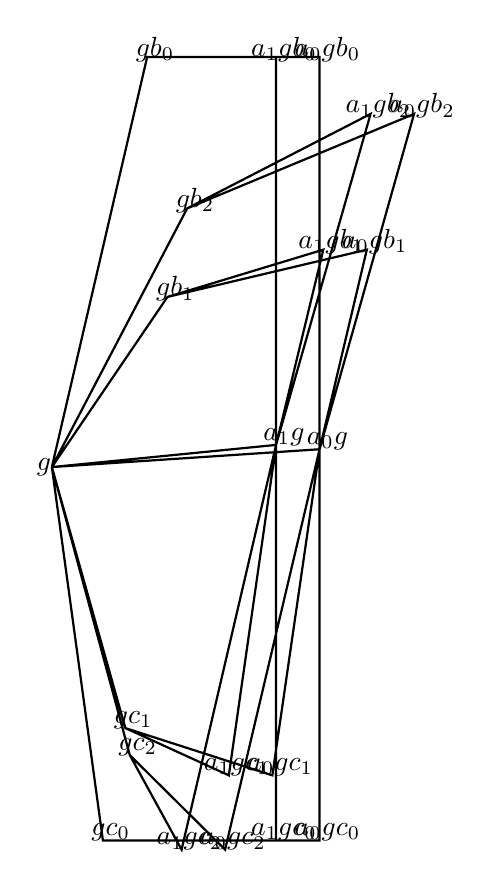
\begin{tikzpicture}
            \draw[thick](0,0)(0,0) -- (1.210143255625387,5.207030998754228) -- (3.3998825955433736,5.207030998754228) -- (3.3998825955433736,0.22635835272529947) -- (0,0)
(0,0) -- (1.4682883024414015,2.16097268112648) -- (3.9998825955433737,2.7609726811264803) -- (3.3998825955433736,0.22635835272529947) -- (0,0)
(0,0) -- (1.7181025748679724,3.284888127730613) -- (4.599882595543374,4.4848881277306125) -- (3.3998825955433736,0.22635835272529947) -- (0,0)
(0,0) -- (1.210143255625387,5.207030998754228) -- (2.8474559653795204,5.207030998754228) -- (2.8474559653795204,0.2814660781474985) -- (0,0)
(0,0) -- (1.4682883024414015,2.16097268112648) -- (3.4474559653795205,2.7609726811264803) -- (2.8474559653795204,0.2814660781474985) -- (0,0)
(0,0) -- (1.7181025748679724,3.284888127730613) -- (4.047455965379521,4.4848881277306125) -- (2.8474559653795204,0.2814660781474985) -- (0,0)
(0,0) -- (0.6480730678270592,-4.741222292613488) -- (3.3998825955433736,-4.741222292613488) -- (3.3998825955433736,0.22635835272529947) -- (0,0)
(0,0) -- (0.9334161679932669,-3.3150013298669014) -- (2.7998825955433735,-3.9150013298669015) -- (3.3998825955433736,0.22635835272529947) -- (0,0)
(0,0) -- (0.9898235486559122,-3.6581096707857936) -- (2.1998825955433734,-4.858109670785794) -- (3.3998825955433736,0.22635835272529947) -- (0,0)
(0,0) -- (0.6480730678270592,-4.741222292613488) -- (2.8474559653795204,-4.741222292613488) -- (2.8474559653795204,0.2814660781474985) -- (0,0)
(0,0) -- (0.9334161679932669,-3.3150013298669014) -- (2.2474559653795203,-3.9150013298669015) -- (2.8474559653795204,0.2814660781474985) -- (0,0)
(0,0) -- (0.9898235486559122,-3.6581096707857936) -- (1.6474559653795204,-4.858109670785794) -- (2.8474559653795204,0.2814660781474985) -- (0,0)
;
\node at (3.4998825955433737,5.307030998754228) {$ a_{ 0  } gb_{ 0 } $};
\node at (4.099882595543374,2.8609726811264804) {$ a_{ 0  } gb_{ 1 } $};
\node at (4.699882595543373,4.584888127730612) {$ a_{ 0  } gb_{ 2 } $};
\node at (2.9474559653795205,5.307030998754228) {$ a_{ 1  } gb_{ 0 } $};
\node at (3.5474559653795206,2.8609726811264804) {$ a_{ 1  } gb_{ 1 } $};
\node at (4.14745596537952,4.584888127730612) {$ a_{ 1  } gb_{ 2 } $};
\node at (3.4998825955433737,-4.641222292613488) {$ a_{ 0  } gc_{ 0 } $};
\node at (2.8998825955433736,-3.8150013298669014) {$ a_{ 0  } gc_{ 1 } $};
\node at (2.2998825955433735,-4.758109670785794) {$ a_{ 0  } gc_{ 2 } $};
\node at (2.9474559653795205,-4.641222292613488) {$ a_{ 1  } gc_{ 0 } $};
\node at (2.3474559653795204,-3.8150013298669014) {$ a_{ 1  } gc_{ 1 } $};
\node at (1.7474559653795205,-4.758109670785794) {$ a_{ 1  } gc_{ 2 } $};
\node at (-0.1,0) {$ g $};
\node at (3.4998825955433737,0.32635835272529945) {$ a_{ 0 }g $};
\node at (2.9474559653795205,0.38146607814749856) {$ a_{ 1 }g $};
\node at (1.3101432556253871,5.307030998754228) {$ gb_{ 0 } $};
\node at (1.5682883024414016,2.2609726811264803) {$ gb_{ 1 } $};
\node at (1.8181025748679724,3.384888127730613) {$ gb_{ 2 } $};
\node at (0.7480730678270592,-4.641222292613488) {$ gc_{ 0 } $};
\node at (1.033416167993267,-3.2150013298669013) {$ gc_{ 1 } $};
\node at (1.0898235486559122,-3.5581096707857935) {$ gc_{ 2 } $};

            \end{tikzpicture}
            \end{center}
            \caption{Square of the complex, with edges $(g,ag), (agb, gb) \in E_A,
            (g,gb), (agb, ag) \in E_B.$ \label{fig:square}
            }
            \end{figure}
 \begin{figure}[H]
            %\label{fig:square}
            \begin{center}
            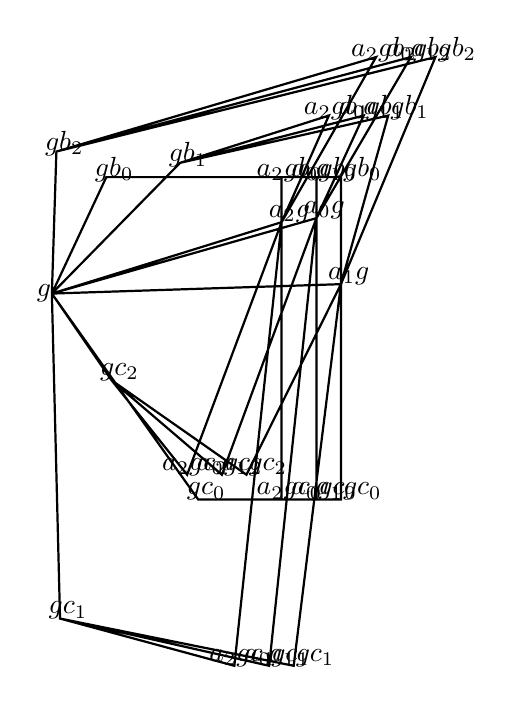
\begin{tikzpicture}
            \draw[thick](0,0)(0,0) -- (0.6913694258279499,1.478690800755841) -- (3.359572905121024,1.478690800755841) -- (3.359572905121024,0.9576137776972984) -- (0,0)
(0,0) -- (1.6289545998057569,1.6603121454780359) -- (3.959572905121024,2.2603121454780357) -- (3.359572905121024,0.9576137776972984) -- (0,0)
(0,0) -- (0.05747747280238524,1.8034142113233194) -- (4.559572905121024,3.003414211323319) -- (3.359572905121024,0.9576137776972984) -- (0,0)
(0,0) -- (0.6913694258279499,1.478690800755841) -- (3.6711623431753093,1.478690800755841) -- (3.6711623431753093,0.11935709406912265) -- (0,0)
(0,0) -- (1.6289545998057569,1.6603121454780359) -- (4.271162343175309,2.2603121454780357) -- (3.6711623431753093,0.11935709406912265) -- (0,0)
(0,0) -- (0.05747747280238524,1.8034142113233194) -- (4.8711623431753095,3.003414211323319) -- (3.6711623431753093,0.11935709406912265) -- (0,0)
(0,0) -- (0.6913694258279499,1.478690800755841) -- (2.9176016387704813,1.478690800755841) -- (2.9176016387704813,0.9064178217784211) -- (0,0)
(0,0) -- (1.6289545998057569,1.6603121454780359) -- (3.5176016387704814,2.2603121454780357) -- (2.9176016387704813,0.9064178217784211) -- (0,0)
(0,0) -- (0.05747747280238524,1.8034142113233194) -- (4.1176016387704815,3.003414211323319) -- (2.9176016387704813,0.9064178217784211) -- (0,0)
(0,0) -- (1.8590757931636042,-2.6161916798438494) -- (3.359572905121024,-2.6161916798438494) -- (3.359572905121024,0.9576137776972984) -- (0,0)
(0,0) -- (0.10370961952579738,-4.127277728473503) -- (2.759572905121024,-4.727277728473503) -- (3.359572905121024,0.9576137776972984) -- (0,0)
(0,0) -- (0.7577615946767449,-1.1007759314717886) -- (2.159572905121024,-2.3007759314717884) -- (3.359572905121024,0.9576137776972984) -- (0,0)
(0,0) -- (1.8590757931636042,-2.6161916798438494) -- (3.6711623431753093,-2.6161916798438494) -- (3.6711623431753093,0.11935709406912265) -- (0,0)
(0,0) -- (0.10370961952579738,-4.127277728473503) -- (3.0711623431753092,-4.727277728473503) -- (3.6711623431753093,0.11935709406912265) -- (0,0)
(0,0) -- (0.7577615946767449,-1.1007759314717886) -- (2.471162343175309,-2.3007759314717884) -- (3.6711623431753093,0.11935709406912265) -- (0,0)
(0,0) -- (1.8590757931636042,-2.6161916798438494) -- (2.9176016387704813,-2.6161916798438494) -- (2.9176016387704813,0.9064178217784211) -- (0,0)
(0,0) -- (0.10370961952579738,-4.127277728473503) -- (2.317601638770481,-4.727277728473503) -- (2.9176016387704813,0.9064178217784211) -- (0,0)
(0,0) -- (0.7577615946767449,-1.1007759314717886) -- (1.7176016387704813,-2.3007759314717884) -- (2.9176016387704813,0.9064178217784211) -- (0,0)
;
\node at (3.459572905121024,1.5786908007558411) {$ a_{ 0  } gb_{ 0 } $};
\node at (4.059572905121024,2.360312145478036) {$ a_{ 0  } gb_{ 1 } $};
\node at (4.659572905121023,3.103414211323319) {$ a_{ 0  } gb_{ 2 } $};
\node at (3.7711623431753094,1.5786908007558411) {$ a_{ 1  } gb_{ 0 } $};
\node at (4.371162343175309,2.360312145478036) {$ a_{ 1  } gb_{ 1 } $};
\node at (4.971162343175309,3.103414211323319) {$ a_{ 1  } gb_{ 2 } $};
\node at (3.0176016387704814,1.5786908007558411) {$ a_{ 2  } gb_{ 0 } $};
\node at (3.6176016387704815,2.360312145478036) {$ a_{ 2  } gb_{ 1 } $};
\node at (4.217601638770481,3.103414211323319) {$ a_{ 2  } gb_{ 2 } $};
\node at (3.459572905121024,-2.5161916798438493) {$ a_{ 0  } gc_{ 0 } $};
\node at (2.859572905121024,-4.627277728473503) {$ a_{ 0  } gc_{ 1 } $};
\node at (2.2595729051210243,-2.2007759314717883) {$ a_{ 0  } gc_{ 2 } $};
\node at (3.7711623431753094,-2.5161916798438493) {$ a_{ 1  } gc_{ 0 } $};
\node at (3.1711623431753093,-4.627277728473503) {$ a_{ 1  } gc_{ 1 } $};
\node at (2.5711623431753092,-2.2007759314717883) {$ a_{ 1  } gc_{ 2 } $};
\node at (3.0176016387704814,-2.5161916798438493) {$ a_{ 2  } gc_{ 0 } $};
\node at (2.4176016387704813,-4.627277728473503) {$ a_{ 2  } gc_{ 1 } $};
\node at (1.8176016387704814,-2.2007759314717883) {$ a_{ 2  } gc_{ 2 } $};
\node at (-0.1,0) {$ g $};
\node at (3.459572905121024,1.0576137776972985) {$ a_{ 0 }g $};
\node at (3.7711623431753094,0.21935709406912265) {$ a_{ 1 }g $};
\node at (3.0176016387704814,1.0064178217784212) {$ a_{ 2 }g $};
\node at (0.7913694258279499,1.5786908007558411) {$ gb_{ 0 } $};
\node at (1.728954599805757,1.760312145478036) {$ gb_{ 1 } $};
\node at (0.15747747280238525,1.9034142113233194) {$ gb_{ 2 } $};
\node at (1.9590757931636043,-2.5161916798438493) {$ gc_{ 0 } $};
\node at (0.2037096195257974,-4.0272777284735035) {$ gc_{ 1 } $};
\node at (0.8577615946767448,-1.0007759314717886) {$ gc_{ 2 } $};

            \end{tikzpicture}
            \end{center}
            \caption{Square of the complex, with edges $(g,ag), (agb, gb) \in E_A,
            (g,gb), (agb, ag) \in E_B.$ \label{fig:square}
            }
            \end{figure}
 \begin{figure}[H]
            %\label{fig:square}
            \begin{center}
            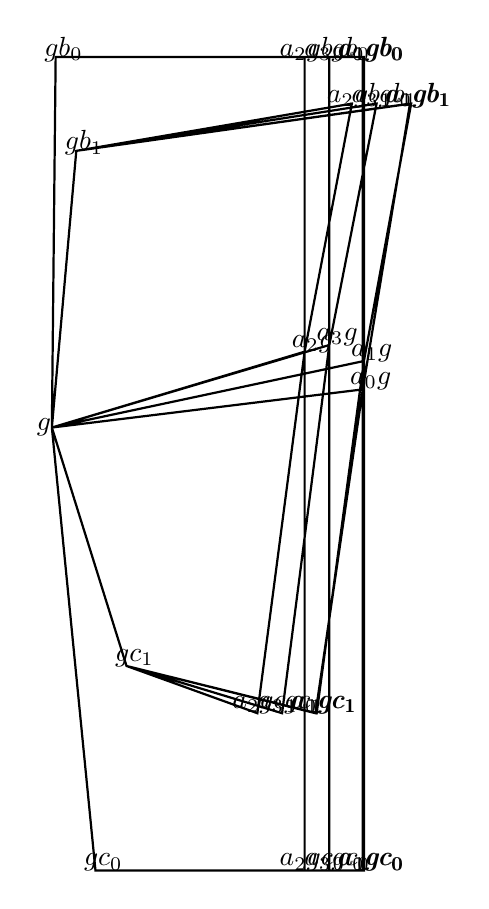
\begin{tikzpicture}
            \draw[thick](0,0)(0,0) -- (0.04802666037906156,4.704950393020561) -- (3.948182137925231,4.704950393020561) -- (3.948182137925231,0.4844140108355732) -- (0,0)
(0,0) -- (0.31018469058539044,3.5136977590662375) -- (4.548182137925231,4.113697759066238) -- (3.948182137925231,0.4844140108355732) -- (0,0)
(0,0) -- (0.04802666037906156,4.704950393020561) -- (3.962974684441818,4.704950393020561) -- (3.962974684441818,0.8448620156880836) -- (0,0)
(0,0) -- (0.31018469058539044,3.5136977590662375) -- (4.5629746844418175,4.113697759066238) -- (3.962974684441818,0.8448620156880836) -- (0,0)
(0,0) -- (0.04802666037906156,4.704950393020561) -- (3.2097417654502416,4.704950393020561) -- (3.2097417654502416,0.963331335145419) -- (0,0)
(0,0) -- (0.31018469058539044,3.5136977590662375) -- (3.8097417654502417,4.113697759066238) -- (3.2097417654502416,0.963331335145419) -- (0,0)
(0,0) -- (0.04802666037906156,4.704950393020561) -- (3.523584658240847,4.704950393020561) -- (3.523584658240847,1.0480181701537845) -- (0,0)
(0,0) -- (0.31018469058539044,3.5136977590662375) -- (4.123584658240847,4.113697759066238) -- (3.523584658240847,1.0480181701537845) -- (0,0)
(0,0) -- (0.5537587923177656,-5.626069730688806) -- (3.948182137925231,-5.626069730688806) -- (3.948182137925231,0.4844140108355732) -- (0,0)
(0,0) -- (0.94807481151409,-3.0279481843953775) -- (3.348182137925231,-3.6279481843953776) -- (3.948182137925231,0.4844140108355732) -- (0,0)
(0,0) -- (0.5537587923177656,-5.626069730688806) -- (3.962974684441818,-5.626069730688806) -- (3.962974684441818,0.8448620156880836) -- (0,0)
(0,0) -- (0.94807481151409,-3.0279481843953775) -- (3.362974684441818,-3.6279481843953776) -- (3.962974684441818,0.8448620156880836) -- (0,0)
(0,0) -- (0.5537587923177656,-5.626069730688806) -- (3.2097417654502416,-5.626069730688806) -- (3.2097417654502416,0.963331335145419) -- (0,0)
(0,0) -- (0.94807481151409,-3.0279481843953775) -- (2.6097417654502415,-3.6279481843953776) -- (3.2097417654502416,0.963331335145419) -- (0,0)
(0,0) -- (0.5537587923177656,-5.626069730688806) -- (3.523584658240847,-5.626069730688806) -- (3.523584658240847,1.0480181701537845) -- (0,0)
(0,0) -- (0.94807481151409,-3.0279481843953775) -- (2.923584658240847,-3.6279481843953776) -- (3.523584658240847,1.0480181701537845) -- (0,0)
;
\node at (4.048182137925231,4.804950393020561) {$ a_{ 0  } gb_{ 0 } $};
\node at (4.648182137925231,4.213697759066237) {$ a_{ 0  } gb_{ 1 } $};
\node at (4.0629746844418175,4.804950393020561) {$ a_{ 1  } gb_{ 0 } $};
\node at (4.662974684441817,4.213697759066237) {$ a_{ 1  } gb_{ 1 } $};
\node at (3.3097417654502417,4.804950393020561) {$ a_{ 2  } gb_{ 0 } $};
\node at (3.9097417654502418,4.213697759066237) {$ a_{ 2  } gb_{ 1 } $};
\node at (3.6235846582408473,4.804950393020561) {$ a_{ 3  } gb_{ 0 } $};
\node at (4.2235846582408465,4.213697759066237) {$ a_{ 3  } gb_{ 1 } $};
\node at (4.048182137925231,-5.526069730688806) {$ a_{ 0  } gc_{ 0 } $};
\node at (3.448182137925231,-3.5279481843953775) {$ a_{ 0  } gc_{ 1 } $};
\node at (4.0629746844418175,-5.526069730688806) {$ a_{ 1  } gc_{ 0 } $};
\node at (3.462974684441818,-3.5279481843953775) {$ a_{ 1  } gc_{ 1 } $};
\node at (3.3097417654502417,-5.526069730688806) {$ a_{ 2  } gc_{ 0 } $};
\node at (2.7097417654502416,-3.5279481843953775) {$ a_{ 2  } gc_{ 1 } $};
\node at (3.6235846582408473,-5.526069730688806) {$ a_{ 3  } gc_{ 0 } $};
\node at (3.023584658240847,-3.5279481843953775) {$ a_{ 3  } gc_{ 1 } $};
\node at (-0.1,0) {$ g $};
\node at (4.048182137925231,0.5844140108355732) {$ a_{ 0 }g $};
\node at (4.0629746844418175,0.9448620156880836) {$ a_{ 1 }g $};
\node at (3.3097417654502417,1.063331335145419) {$ a_{ 2 }g $};
\node at (3.6235846582408473,1.1480181701537846) {$ a_{ 3 }g $};
\node at (0.14802666037906156,4.804950393020561) {$ gb_{ 0 } $};
\node at (0.4101846905853904,3.6136977590662376) {$ gb_{ 1 } $};
\node at (0.6537587923177656,-5.526069730688806) {$ gc_{ 0 } $};
\node at (1.04807481151409,-2.9279481843953774) {$ gc_{ 1 } $};

            \end{tikzpicture}
            \end{center}
            \caption{Square of the complex, with edges $(g,ag), (agb, gb) \in E_A,
            (g,gb), (agb, ag) \in E_B.$ \label{fig:square}
            }
            \end{figure}
 \begin{figure}[H]
            %\label{fig:square}
            \begin{center}
            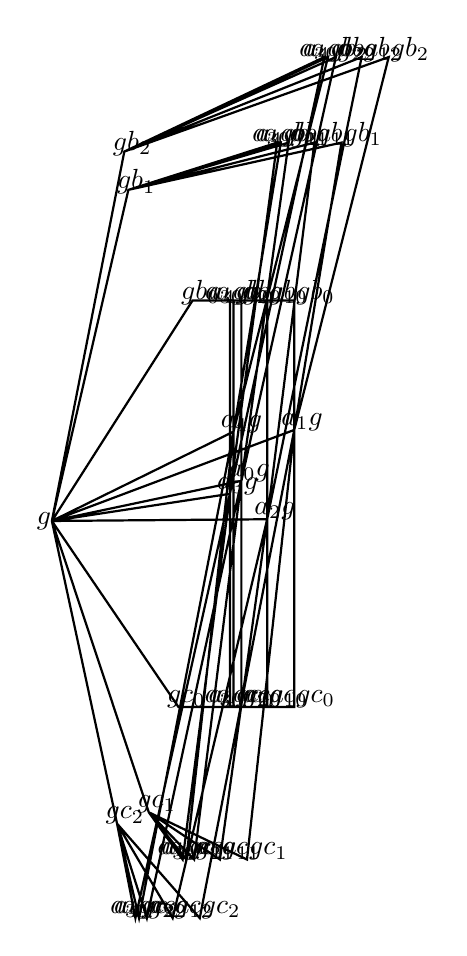
\begin{tikzpicture}
            \draw[thick](0,0)(0,0) -- (1.7871905477244538,2.800486803294876) -- (2.4066120820288743,2.800486803294876) -- (2.4066120820288743,0.5093206263560092) -- (0,0)
(0,0) -- (0.9717049024621869,4.204990573237014) -- (3.0066120820288744,4.8049905732370135) -- (2.4066120820288743,0.5093206263560092) -- (0,0)
(0,0) -- (0.9201285665575163,4.691471676092082) -- (3.6066120820288745,5.891471676092082) -- (2.4066120820288743,0.5093206263560092) -- (0,0)
(0,0) -- (1.7871905477244538,2.800486803294876) -- (3.0780613160100696,2.800486803294876) -- (3.0780613160100696,1.1562827298369682) -- (0,0)
(0,0) -- (0.9717049024621869,4.204990573237014) -- (3.6780613160100697,4.8049905732370135) -- (3.0780613160100696,1.1562827298369682) -- (0,0)
(0,0) -- (0.9201285665575163,4.691471676092082) -- (4.27806131601007,5.891471676092082) -- (3.0780613160100696,1.1562827298369682) -- (0,0)
(0,0) -- (1.7871905477244538,2.800486803294876) -- (2.7341003235670582,2.800486803294876) -- (2.7341003235670582,0.021828772594230106) -- (0,0)
(0,0) -- (0.9717049024621869,4.204990573237014) -- (3.3341003235670583,4.8049905732370135) -- (2.7341003235670582,0.021828772594230106) -- (0,0)
(0,0) -- (0.9201285665575163,4.691471676092082) -- (3.9341003235670584,5.891471676092082) -- (2.7341003235670582,0.021828772594230106) -- (0,0)
(0,0) -- (1.7871905477244538,2.800486803294876) -- (2.260945754412379,2.800486803294876) -- (2.260945754412379,0.34506776086479346) -- (0,0)
(0,0) -- (0.9717049024621869,4.204990573237014) -- (2.8609457544123793,4.8049905732370135) -- (2.260945754412379,0.34506776086479346) -- (0,0)
(0,0) -- (0.9201285665575163,4.691471676092082) -- (3.4609457544123794,5.891471676092082) -- (2.260945754412379,0.34506776086479346) -- (0,0)
(0,0) -- (1.7871905477244538,2.800486803294876) -- (2.307173625345933,2.800486803294876) -- (2.307173625345933,1.1347804442751708) -- (0,0)
(0,0) -- (0.9717049024621869,4.204990573237014) -- (2.907173625345933,4.8049905732370135) -- (2.307173625345933,1.1347804442751708) -- (0,0)
(0,0) -- (0.9201285665575163,4.691471676092082) -- (3.507173625345933,5.891471676092082) -- (2.307173625345933,1.1347804442751708) -- (0,0)
(0,0) -- (1.607203874835598,-2.361676819900966) -- (2.4066120820288743,-2.361676819900966) -- (2.4066120820288743,0.5093206263560092) -- (0,0)
(0,0) -- (1.2305357392329097,-3.699550046136711) -- (1.8066120820288742,-4.29955004613671) -- (2.4066120820288743,0.5093206263560092) -- (0,0)
(0,0) -- (0.8277694284288124,-3.8433913473509738) -- (1.2066120820288744,-5.0433913473509735) -- (2.4066120820288743,0.5093206263560092) -- (0,0)
(0,0) -- (1.607203874835598,-2.361676819900966) -- (3.0780613160100696,-2.361676819900966) -- (3.0780613160100696,1.1562827298369682) -- (0,0)
(0,0) -- (1.2305357392329097,-3.699550046136711) -- (2.4780613160100695,-4.29955004613671) -- (3.0780613160100696,1.1562827298369682) -- (0,0)
(0,0) -- (0.8277694284288124,-3.8433913473509738) -- (1.8780613160100696,-5.0433913473509735) -- (3.0780613160100696,1.1562827298369682) -- (0,0)
(0,0) -- (1.607203874835598,-2.361676819900966) -- (2.7341003235670582,-2.361676819900966) -- (2.7341003235670582,0.021828772594230106) -- (0,0)
(0,0) -- (1.2305357392329097,-3.699550046136711) -- (2.134100323567058,-4.29955004613671) -- (2.7341003235670582,0.021828772594230106) -- (0,0)
(0,0) -- (0.8277694284288124,-3.8433913473509738) -- (1.5341003235670583,-5.0433913473509735) -- (2.7341003235670582,0.021828772594230106) -- (0,0)
(0,0) -- (1.607203874835598,-2.361676819900966) -- (2.260945754412379,-2.361676819900966) -- (2.260945754412379,0.34506776086479346) -- (0,0)
(0,0) -- (1.2305357392329097,-3.699550046136711) -- (1.6609457544123791,-4.29955004613671) -- (2.260945754412379,0.34506776086479346) -- (0,0)
(0,0) -- (0.8277694284288124,-3.8433913473509738) -- (1.0609457544123793,-5.0433913473509735) -- (2.260945754412379,0.34506776086479346) -- (0,0)
(0,0) -- (1.607203874835598,-2.361676819900966) -- (2.307173625345933,-2.361676819900966) -- (2.307173625345933,1.1347804442751708) -- (0,0)
(0,0) -- (1.2305357392329097,-3.699550046136711) -- (1.7071736253459329,-4.29955004613671) -- (2.307173625345933,1.1347804442751708) -- (0,0)
(0,0) -- (0.8277694284288124,-3.8433913473509738) -- (1.107173625345933,-5.0433913473509735) -- (2.307173625345933,1.1347804442751708) -- (0,0)
;
\node at (2.5066120820288744,2.9004868032948763) {$ a_{ 0  } gb_{ 0 } $};
\node at (3.1066120820288745,4.904990573237013) {$ a_{ 0  } gb_{ 1 } $};
\node at (3.7066120820288746,5.991471676092082) {$ a_{ 0  } gb_{ 2 } $};
\node at (3.1780613160100697,2.9004868032948763) {$ a_{ 1  } gb_{ 0 } $};
\node at (3.77806131601007,4.904990573237013) {$ a_{ 1  } gb_{ 1 } $};
\node at (4.378061316010069,5.991471676092082) {$ a_{ 1  } gb_{ 2 } $};
\node at (2.8341003235670583,2.9004868032948763) {$ a_{ 2  } gb_{ 0 } $};
\node at (3.4341003235670584,4.904990573237013) {$ a_{ 2  } gb_{ 1 } $};
\node at (4.034100323567058,5.991471676092082) {$ a_{ 2  } gb_{ 2 } $};
\node at (2.3609457544123793,2.9004868032948763) {$ a_{ 3  } gb_{ 0 } $};
\node at (2.9609457544123794,4.904990573237013) {$ a_{ 3  } gb_{ 1 } $};
\node at (3.5609457544123795,5.991471676092082) {$ a_{ 3  } gb_{ 2 } $};
\node at (2.407173625345933,2.9004868032948763) {$ a_{ 4  } gb_{ 0 } $};
\node at (3.007173625345933,4.904990573237013) {$ a_{ 4  } gb_{ 1 } $};
\node at (3.607173625345933,5.991471676092082) {$ a_{ 4  } gb_{ 2 } $};
\node at (2.5066120820288744,-2.261676819900966) {$ a_{ 0  } gc_{ 0 } $};
\node at (1.9066120820288743,-4.199550046136711) {$ a_{ 0  } gc_{ 1 } $};
\node at (1.3066120820288745,-4.943391347350974) {$ a_{ 0  } gc_{ 2 } $};
\node at (3.1780613160100697,-2.261676819900966) {$ a_{ 1  } gc_{ 0 } $};
\node at (2.5780613160100696,-4.199550046136711) {$ a_{ 1  } gc_{ 1 } $};
\node at (1.9780613160100697,-4.943391347350974) {$ a_{ 1  } gc_{ 2 } $};
\node at (2.8341003235670583,-2.261676819900966) {$ a_{ 2  } gc_{ 0 } $};
\node at (2.2341003235670582,-4.199550046136711) {$ a_{ 2  } gc_{ 1 } $};
\node at (1.6341003235670584,-4.943391347350974) {$ a_{ 2  } gc_{ 2 } $};
\node at (2.3609457544123793,-2.261676819900966) {$ a_{ 3  } gc_{ 0 } $};
\node at (1.7609457544123792,-4.199550046136711) {$ a_{ 3  } gc_{ 1 } $};
\node at (1.1609457544123793,-4.943391347350974) {$ a_{ 3  } gc_{ 2 } $};
\node at (2.407173625345933,-2.261676819900966) {$ a_{ 4  } gc_{ 0 } $};
\node at (1.807173625345933,-4.199550046136711) {$ a_{ 4  } gc_{ 1 } $};
\node at (1.207173625345933,-4.943391347350974) {$ a_{ 4  } gc_{ 2 } $};
\node at (-0.1,0) {$ g $};
\node at (2.5066120820288744,0.6093206263560091) {$ a_{ 0 }g $};
\node at (3.1780613160100697,1.2562827298369683) {$ a_{ 1 }g $};
\node at (2.8341003235670583,0.12182877259423011) {$ a_{ 2 }g $};
\node at (2.3609457544123793,0.4450677608647935) {$ a_{ 3 }g $};
\node at (2.407173625345933,1.2347804442751709) {$ a_{ 4 }g $};
\node at (1.887190547724454,2.9004868032948763) {$ gb_{ 0 } $};
\node at (1.071704902462187,4.3049905732370135) {$ gb_{ 1 } $};
\node at (1.0201285665575164,4.7914716760920815) {$ gb_{ 2 } $};
\node at (1.707203874835598,-2.261676819900966) {$ gc_{ 0 } $};
\node at (1.3305357392329098,-3.5995500461367107) {$ gc_{ 1 } $};
\node at (0.9277694284288124,-3.7433913473509737) {$ gc_{ 2 } $};

            \end{tikzpicture}
            \end{center}
            \caption{Square of the complex, with edges $(g,ag), (agb, gb) \in E_A,
            (g,gb), (agb, ag) \in E_B.$ \label{fig:square}
            }
            \end{figure}
 \begin{figure}[H]
            %\label{fig:square}
            \begin{center}
            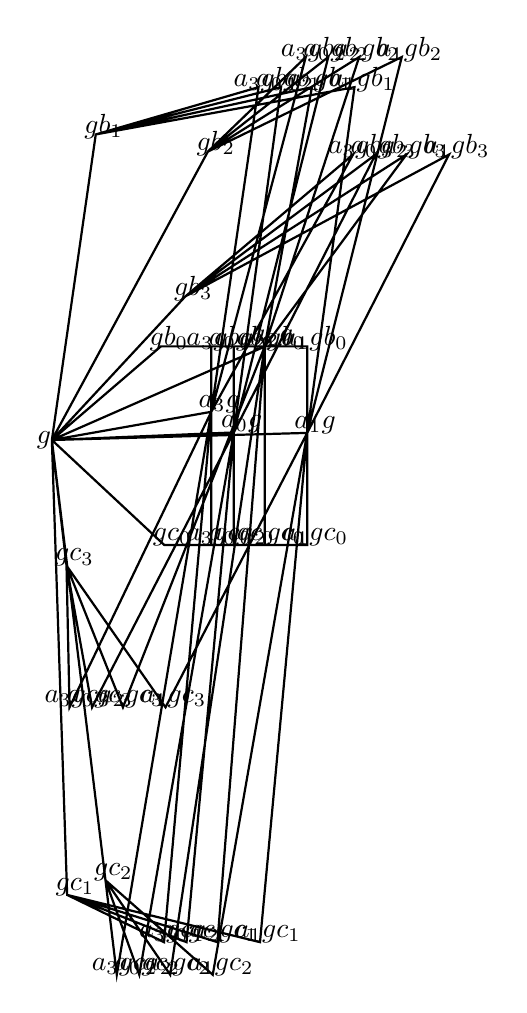
\begin{tikzpicture}
            \draw[thick](0,0)(0,0) -- (1.3851910059761157,1.189333952488699) -- (2.3102227927095553,1.189333952488699) -- (2.3102227927095553,0.09593203033212672) -- (0,0)
(0,0) -- (0.5574999225673178,3.8808501356139056) -- (2.9102227927095554,4.480850135613905) -- (2.3102227927095553,0.09593203033212672) -- (0,0)
(0,0) -- (1.9817974289643214,3.663314605052698) -- (3.5102227927095555,4.863314605052698) -- (2.3102227927095553,0.09593203033212672) -- (0,0)
(0,0) -- (1.696557421166624,1.8247910710538036) -- (4.110222792709555,3.6247910710538034) -- (2.3102227927095553,0.09593203033212672) -- (0,0)
(0,0) -- (1.3851910059761157,1.189333952488699) -- (3.2432139552016928,1.189333952488699) -- (3.2432139552016928,0.09025174393620583) -- (0,0)
(0,0) -- (0.5574999225673178,3.8808501356139056) -- (3.843213955201693,4.480850135613905) -- (3.2432139552016928,0.09025174393620583) -- (0,0)
(0,0) -- (1.9817974289643214,3.663314605052698) -- (4.443213955201693,4.863314605052698) -- (3.2432139552016928,0.09025174393620583) -- (0,0)
(0,0) -- (1.696557421166624,1.8247910710538036) -- (5.043213955201693,3.6247910710538034) -- (3.2432139552016928,0.09025174393620583) -- (0,0)
(0,0) -- (1.3851910059761157,1.189333952488699) -- (2.7026158110735494,1.189333952488699) -- (2.7026158110735494,1.1865234132857891) -- (0,0)
(0,0) -- (0.5574999225673178,3.8808501356139056) -- (3.3026158110735495,4.480850135613905) -- (2.7026158110735494,1.1865234132857891) -- (0,0)
(0,0) -- (1.9817974289643214,3.663314605052698) -- (3.9026158110735496,4.863314605052698) -- (2.7026158110735494,1.1865234132857891) -- (0,0)
(0,0) -- (1.696557421166624,1.8247910710538036) -- (4.502615811073549,3.6247910710538034) -- (2.7026158110735494,1.1865234132857891) -- (0,0)
(0,0) -- (1.3851910059761157,1.189333952488699) -- (2.024468469727495,1.189333952488699) -- (2.024468469727495,0.35817309142405357) -- (0,0)
(0,0) -- (0.5574999225673178,3.8808501356139056) -- (2.624468469727495,4.480850135613905) -- (2.024468469727495,0.35817309142405357) -- (0,0)
(0,0) -- (1.9817974289643214,3.663314605052698) -- (3.224468469727495,4.863314605052698) -- (2.024468469727495,0.35817309142405357) -- (0,0)
(0,0) -- (1.696557421166624,1.8247910710538036) -- (3.8244684697274947,3.6247910710538034) -- (2.024468469727495,0.35817309142405357) -- (0,0)
(0,0) -- (1.4286691048874665,-1.334088712806568) -- (2.3102227927095553,-1.334088712806568) -- (2.3102227927095553,0.09593203033212672) -- (0,0)
(0,0) -- (0.19400615050094316,-5.7772772427804036) -- (1.7102227927095552,-6.377277242780403) -- (2.3102227927095553,0.09593203033212672) -- (0,0)
(0,0) -- (0.6809459933709143,-5.59111500419274) -- (1.1102227927095554,-6.79111500419274) -- (2.3102227927095553,0.09593203033212672) -- (0,0)
(0,0) -- (0.1858492158187759,-1.5943442754704076) -- (0.5102227927095555,-3.3943442754704076) -- (2.3102227927095553,0.09593203033212672) -- (0,0)
(0,0) -- (1.4286691048874665,-1.334088712806568) -- (3.2432139552016928,-1.334088712806568) -- (3.2432139552016928,0.09025174393620583) -- (0,0)
(0,0) -- (0.19400615050094316,-5.7772772427804036) -- (2.6432139552016927,-6.377277242780403) -- (3.2432139552016928,0.09025174393620583) -- (0,0)
(0,0) -- (0.6809459933709143,-5.59111500419274) -- (2.0432139552016926,-6.79111500419274) -- (3.2432139552016928,0.09025174393620583) -- (0,0)
(0,0) -- (0.1858492158187759,-1.5943442754704076) -- (1.443213955201693,-3.3943442754704076) -- (3.2432139552016928,0.09025174393620583) -- (0,0)
(0,0) -- (1.4286691048874665,-1.334088712806568) -- (2.7026158110735494,-1.334088712806568) -- (2.7026158110735494,1.1865234132857891) -- (0,0)
(0,0) -- (0.19400615050094316,-5.7772772427804036) -- (2.1026158110735493,-6.377277242780403) -- (2.7026158110735494,1.1865234132857891) -- (0,0)
(0,0) -- (0.6809459933709143,-5.59111500419274) -- (1.5026158110735495,-6.79111500419274) -- (2.7026158110735494,1.1865234132857891) -- (0,0)
(0,0) -- (0.1858492158187759,-1.5943442754704076) -- (0.9026158110735496,-3.3943442754704076) -- (2.7026158110735494,1.1865234132857891) -- (0,0)
(0,0) -- (1.4286691048874665,-1.334088712806568) -- (2.024468469727495,-1.334088712806568) -- (2.024468469727495,0.35817309142405357) -- (0,0)
(0,0) -- (0.19400615050094316,-5.7772772427804036) -- (1.4244684697274947,-6.377277242780403) -- (2.024468469727495,0.35817309142405357) -- (0,0)
(0,0) -- (0.6809459933709143,-5.59111500419274) -- (0.8244684697274949,-6.79111500419274) -- (2.024468469727495,0.35817309142405357) -- (0,0)
(0,0) -- (0.1858492158187759,-1.5943442754704076) -- (0.224468469727495,-3.3943442754704076) -- (2.024468469727495,0.35817309142405357) -- (0,0)
;
\node at (2.4102227927095554,1.289333952488699) {$ a_{ 0  } gb_{ 0 } $};
\node at (3.0102227927095555,4.580850135613905) {$ a_{ 0  } gb_{ 1 } $};
\node at (3.6102227927095556,4.963314605052697) {$ a_{ 0  } gb_{ 2 } $};
\node at (4.210222792709555,3.7247910710538035) {$ a_{ 0  } gb_{ 3 } $};
\node at (3.343213955201693,1.289333952488699) {$ a_{ 1  } gb_{ 0 } $};
\node at (3.943213955201693,4.580850135613905) {$ a_{ 1  } gb_{ 1 } $};
\node at (4.543213955201693,4.963314605052697) {$ a_{ 1  } gb_{ 2 } $};
\node at (5.143213955201692,3.7247910710538035) {$ a_{ 1  } gb_{ 3 } $};
\node at (2.8026158110735495,1.289333952488699) {$ a_{ 2  } gb_{ 0 } $};
\node at (3.4026158110735496,4.580850135613905) {$ a_{ 2  } gb_{ 1 } $};
\node at (4.002615811073549,4.963314605052697) {$ a_{ 2  } gb_{ 2 } $};
\node at (4.602615811073549,3.7247910710538035) {$ a_{ 2  } gb_{ 3 } $};
\node at (2.124468469727495,1.289333952488699) {$ a_{ 3  } gb_{ 0 } $};
\node at (2.724468469727495,4.580850135613905) {$ a_{ 3  } gb_{ 1 } $};
\node at (3.324468469727495,4.963314605052697) {$ a_{ 3  } gb_{ 2 } $};
\node at (3.9244684697274947,3.7247910710538035) {$ a_{ 3  } gb_{ 3 } $};
\node at (2.4102227927095554,-1.2340887128065678) {$ a_{ 0  } gc_{ 0 } $};
\node at (1.8102227927095553,-6.2772772427804036) {$ a_{ 0  } gc_{ 1 } $};
\node at (1.2102227927095555,-6.69111500419274) {$ a_{ 0  } gc_{ 2 } $};
\node at (0.6102227927095555,-3.2943442754704075) {$ a_{ 0  } gc_{ 3 } $};
\node at (3.343213955201693,-1.2340887128065678) {$ a_{ 1  } gc_{ 0 } $};
\node at (2.7432139552016928,-6.2772772427804036) {$ a_{ 1  } gc_{ 1 } $};
\node at (2.1432139552016927,-6.69111500419274) {$ a_{ 1  } gc_{ 2 } $};
\node at (1.543213955201693,-3.2943442754704075) {$ a_{ 1  } gc_{ 3 } $};
\node at (2.8026158110735495,-1.2340887128065678) {$ a_{ 2  } gc_{ 0 } $};
\node at (2.2026158110735494,-6.2772772427804036) {$ a_{ 2  } gc_{ 1 } $};
\node at (1.6026158110735496,-6.69111500419274) {$ a_{ 2  } gc_{ 2 } $};
\node at (1.0026158110735497,-3.2943442754704075) {$ a_{ 2  } gc_{ 3 } $};
\node at (2.124468469727495,-1.2340887128065678) {$ a_{ 3  } gc_{ 0 } $};
\node at (1.5244684697274948,-6.2772772427804036) {$ a_{ 3  } gc_{ 1 } $};
\node at (0.9244684697274949,-6.69111500419274) {$ a_{ 3  } gc_{ 2 } $};
\node at (0.324468469727495,-3.2943442754704075) {$ a_{ 3  } gc_{ 3 } $};
\node at (-0.1,0) {$ g $};
\node at (2.4102227927095554,0.19593203033212672) {$ a_{ 0 }g $};
\node at (3.343213955201693,0.19025174393620584) {$ a_{ 1 }g $};
\node at (2.8026158110735495,1.2865234132857892) {$ a_{ 2 }g $};
\node at (2.124468469727495,0.4581730914240536) {$ a_{ 3 }g $};
\node at (1.4851910059761158,1.289333952488699) {$ gb_{ 0 } $};
\node at (0.6574999225673178,3.9808501356139057) {$ gb_{ 1 } $};
\node at (2.0817974289643213,3.763314605052698) {$ gb_{ 2 } $};
\node at (1.796557421166624,1.9247910710538036) {$ gb_{ 3 } $};
\node at (1.5286691048874665,-1.2340887128065678) {$ gc_{ 0 } $};
\node at (0.29400615050094314,-5.677277242780404) {$ gc_{ 1 } $};
\node at (0.7809459933709143,-5.49111500419274) {$ gc_{ 2 } $};
\node at (0.28584921581877587,-1.4943442754704075) {$ gc_{ 3 } $};

            \end{tikzpicture}
            \end{center}
            \caption{Square of the complex, with edges $(g,ag), (agb, gb) \in E_A,
            (g,gb), (agb, ag) \in E_B.$ \label{fig:square}
            }
            \end{figure}
 
%\end{multicols*}
  % \printbibliography 
\end{document}

 